%-------------------------------------------------------------------------------
\section{Evaluation}
%-------------------------------------------------------------------------------
\subsection{Methodology}
In evaluation, we use a machine with two Intel Xeon Octa-core E5-2640V3 processors(2.6Ghz), 64GB DRAM, and Intel SSD DC S3520 of 480GB. For PM, we use Intel Optane DC 256 GB Persistent Memory Module, and for the operation system, we use Ubuntu 18.04LTS with Linux kernel version 4.15 is used.
We run PC-DB and RocksDB in this platform by contrast. In PC-DB, we use the APP Direct Mode of Intel Optane DC Persistent Memory Module. The MemTable size in RocksDB and PC-DB is set to 64MB, and a fixed key size of 20 byte is used.  All SSTable files are stored in the SSD in both database. 
To evaluate the performance of the two database, we use the db$_$bench benchmarks as microbenchmark and the YCSB as real world workload benchmarks. we execute the benchmark as single-threaded workloads as RocksDB is not optimized for multi-threaded workloads. For each run, a random write workload create the database by inserting 8GB data , where N write operations are performed in total. Then each of the other workloads performs $0.2\times N$ of its own operation against the database.  
\subsection{Using a Persistent MemTable}
Generally our design can be divided into two parts: to get better consistency in exchange of performance, we use PM to replace DRAM; and to improve the read amplification in the validation phase in OCC, we use DRAM to store the outstanding transaction version. In order to better understand what is the effect of the two strategy, we first evaluate the performance of RocksDB,  a modified version of RocksDB by replacing the DRAM using PM, and the PC-DB. Figure 5 shows the expected performance of this evaluation for the random write workload form db$\_$bench over various value sizes. The write latency and total amount of data written to disk is normalized to these of RocksDB.
\begin{figure}
    \centering
    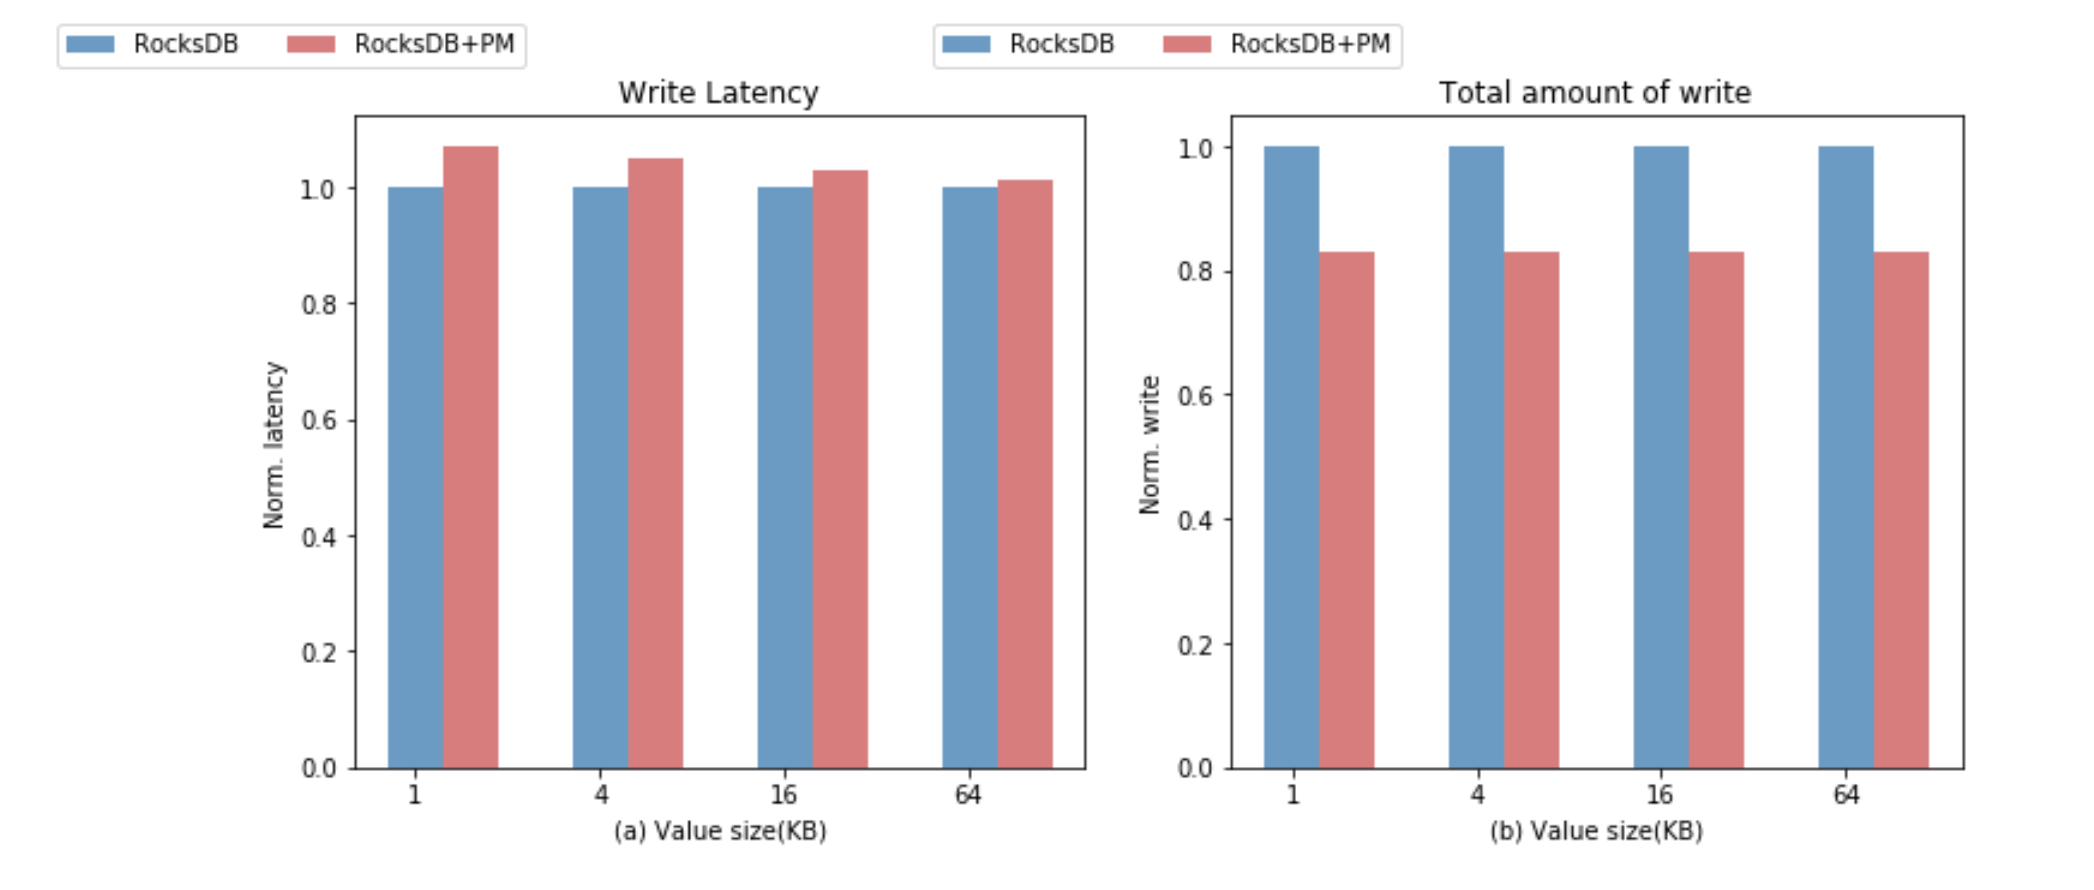
\includegraphics[width=0.36\paperwidth]{USENIX/figure/Randomwrite.png}
    \caption{Random write performance comparison}
    \label{fig:randomwrite}
\end{figure}
In the figure of write latency, the write latency of RocksDB is similar to that of RocksDB+PM. This is because 1)the write and read latency of PM is higher than the DRAM. 2) RocksDB have to flush WAL to the disk constantly, reducing the performance of RocksDB. However, RocksDB+PM can persistent the inserted data as soon as it is inserted to MemTable, and it can also provide stronger durability. As for the figure of total amount of write, RocksDB+PM can reduce the amount of write data by about $16\%$ compared to the result of RocksDB. This is because RocksDB+PM don`t have to write the WAL. 
\subsection{Result with Microbenchmarks}
Figure 6 shows the operation throughputs of random write and random read workloads of PC-DB, and all of them are normalized to these of RocksDB.  For the random read, we first run a random write workload to create the database, and then wait until the compaction process is finished on the database before performing their operations.
For the random write operations, PC-DB provides almost the same throughput as the RocksDB over all the value sizes. As we have talked before, the write performance of RocksDB is almost the same as RocksDB+PM, and the introducing of DRAM has almost no effect of write performance, because we just need to insert or update the version of the records when a transaction is committed. This overhead of this operation is small. 
For the random operations, PC-DB also shows a similar performance as RocksDB. This because the read latency of PM is almost the same as that of DRAM, and if PC-DB can not get the key in PM, it will search the disk for the recoed, just like the RocksDB.
\begin{figure}
    \centering
    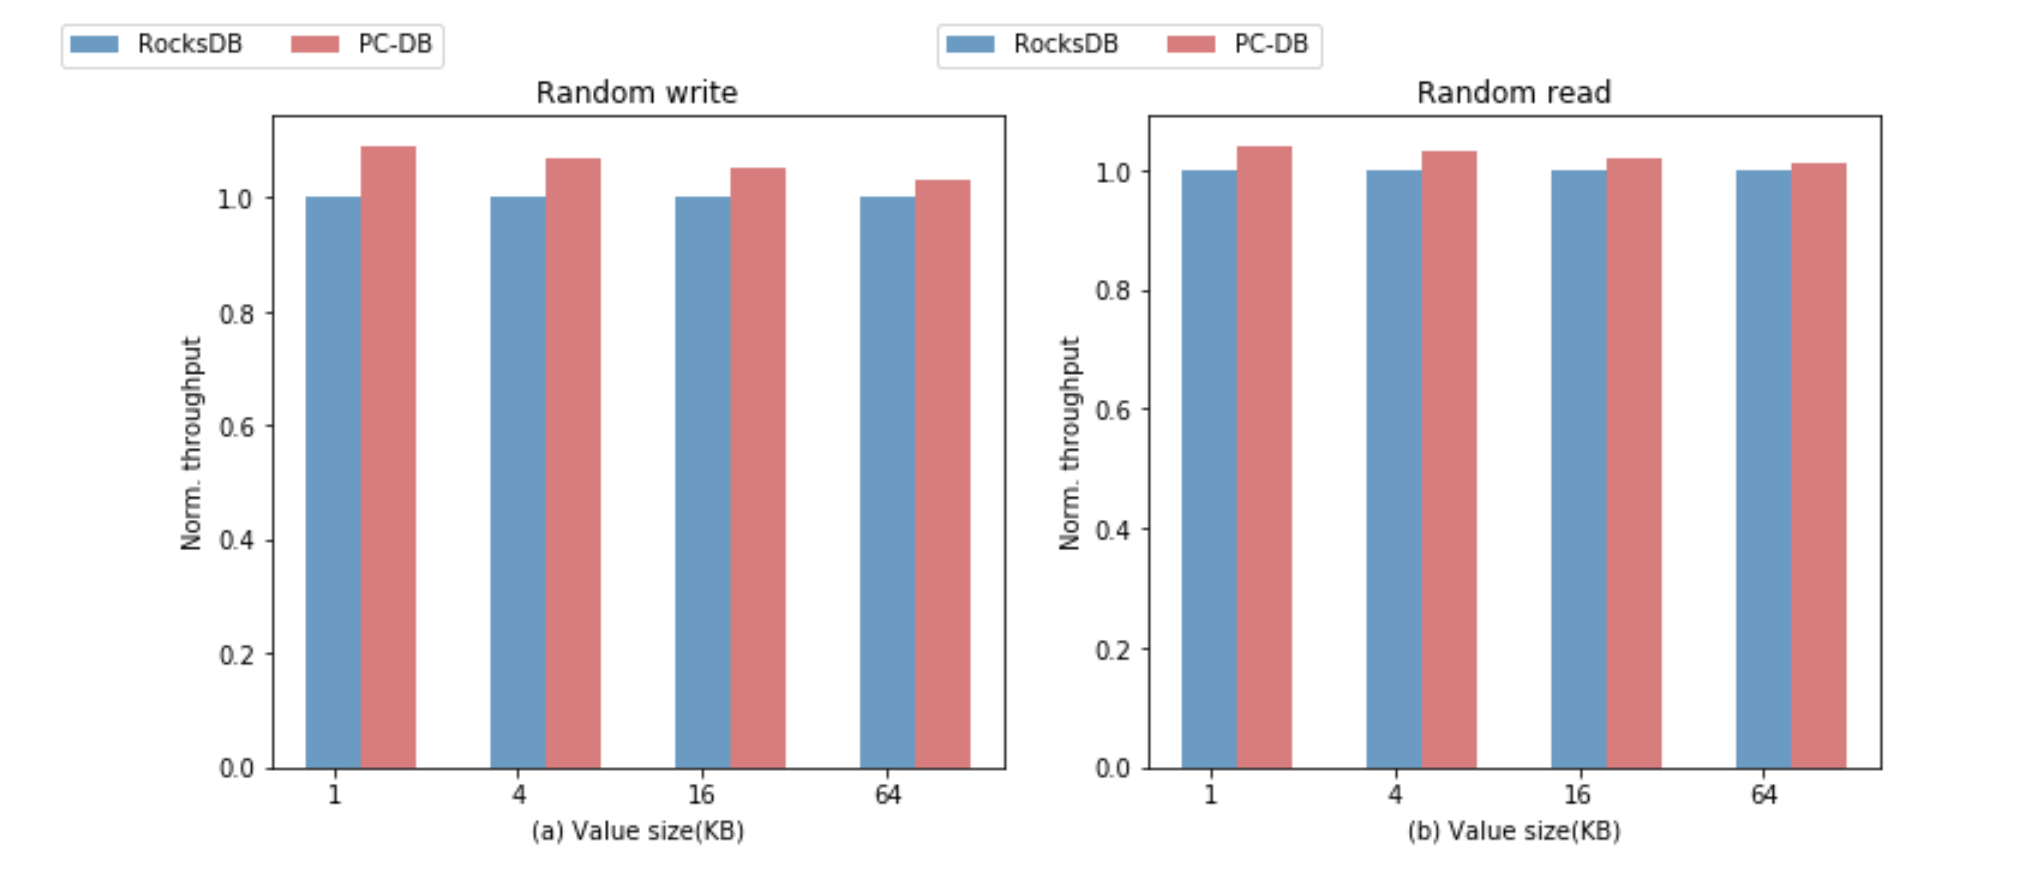
\includegraphics[width=0.36\paperwidth]{USENIX/figure/Throughput.png}
    \caption{Throughput of PC-DB normalized to RocksDB}
    \label{fig:throughput}
\end{figure}
\subsection{Results with YCSB}
YCSB consists of six workloads that capture different real world scenarios. To run the YCSB workloads, we modify db$\_$bench to run YCSB workload traces for various value sizes. Figures 7(a), 7(b) and 7(c) show the operation throughput, latency, and the total amount of write with SLM-DB, normalized to those with RocksDB over the six YCSB workloads [17]. For each workload, the cumulative amount of write is measured when the workload finishes. For the results, we load the database for workload A by inserting KVs, and continuously run workload A, workload B, workload C, workload F, and workload D in order. We then delete the database, and reload the database to run workload E. Workload A performs $50\%$ reads and $50\%$ updates, Workload B performs $95\%$ reads and $5\%$ updates, Workload C performs $100\%$ reads, and Workload F performs $50\%$ reads and $50\%$ read modify-writes. For these workloads, Zipfian distribution is used. Workload D performs $95\%$ reads for the latest keys and $5\%$ inserts. Workload E performs $95\%$ range query and $5\%$ inserts with Zipfian distribution.
\begin{figure}
    \centering
    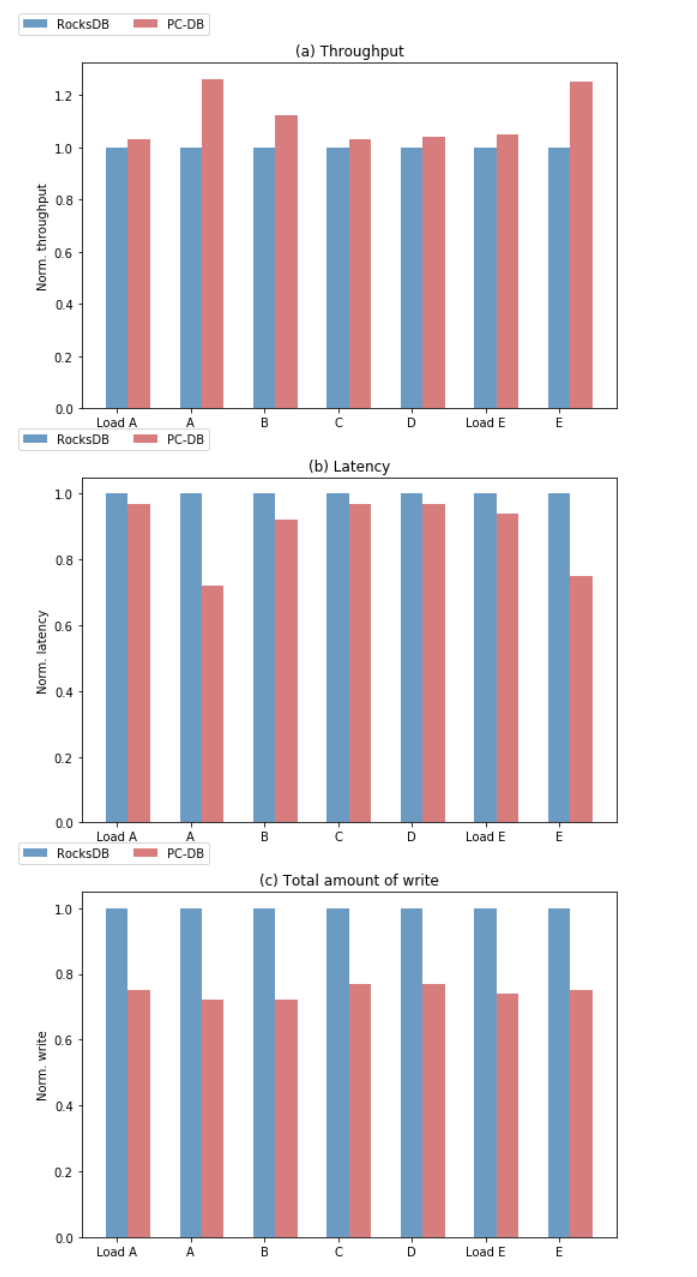
\includegraphics[width=0.36\paperwidth]{USENIX/figure/YCSB performance.png}
    \caption{YCSB performance }
    \label{fig:YCSB}
\end{figure}
In figure $7(a)$ and $7(b)$, the throughput of PC-DB are higher than those of RocksDB and the latency of PC-DB is smaller than the RocksDB for all workloads, which is because of our using of DRAM as the cache. In the validation phase of OCC, we first search the PM for the latest version of a record, and if it is not found, we search it in the DRAM. While in RocksDB, we have to search the disk for the version if it is not found in the DRAM, which will cost a lot. We can also notice that if the write operations have more shares in the total operations, the PC-DB performs better.
In figure $7(c)$, the total amount of write in PC-DB is much smaller than that of RocksDB for all workloads. this is the same reason as the $5.2$: we don`t have to flush WAL in PC-DB.